\section{Cây cú pháp trừu tượng}

Cây cú pháp trừu tượng (Abstract Syntax Tree - AST) là một cấu trúc dữ liệu quan trọng trong ngôn ngữ lập trình Rust, biểu diễn cấu trúc mã nguồn của chương trình. Khi trình biên dịch Rust phân tích mã nguồn, nó tạo ra một AST để hiểu và xử lý cú pháp của chương trình. AST trong Rust giúp trừu tượng hóa các phần chi tiết của mã nguồn và chỉ giữ lại những thông tin cần thiết để trình biên dịch hiểu cấu trúc của chương trình. Điều này bao gồm các thông tin về khai báo biến, hàm, khối lệnh, và các biểu thức khác.

AST trong Rust được sử dụng rộng rãi trong nhiều công cụ và ứng dụng khác nhau, bao gồm trình biên dịch (compiler), trình dịch ngược (decompiler), và các công cụ phân tích mã nguồn (SAST - Source Code Analysis Tool). Trong Rust, AST không chỉ giúp trình biên dịch hiểu cấu trúc của mã nguồn mà còn hỗ trợ quá trình tối ưu hóa và kiểm tra lỗi. Ví dụ, khi Rust kiểm tra các quy tắc về an toàn bộ nhớ, nó sử dụng AST để xác minh rằng các biến được sử dụng đúng cách và không gây ra các lỗi bộ nhớ như tràn bộ đệm hay truy cập ngoài giới hạn.

Đối với các nhà phát triển Rust, việc hiểu và sử dụng AST có thể giúp họ tạo ra các công cụ tùy chỉnh để phân tích và tối ưu hóa mã nguồn. AST cũng hỗ trợ việc thực hiện các thao tác như refactoring, giúp thay đổi cấu trúc mã nguồn một cách tự động mà không làm thay đổi hành vi của chương trình. Ngoài ra, AST còn đóng vai trò quan trọng trong việc tạo ra các công cụ kiểm thử tự động và phân tích bảo mật, giúp phát hiện sớm các lỗi và lỗ hổng tiềm ẩn trong mã nguồn.

Cấu trúc của AST trong Rust có thể khác nhau tùy thuộc vào cách triển khai của trình biên dịch. Mỗi nút trong AST đại diện cho một phần tử cụ thể của mã nguồn, chẳng hạn như một khai báo biến hay một biểu thức điều kiện. Các nút này có thể có các thuộc tính và con trỏ đến các nút con, tạo thành một cây cấu trúc phân cấp.

Một trong những ưu điểm lớn của AST trong Rust là khả năng tích hợp với các công cụ xử lý ngôn ngữ tự nhiên (NLP) và các công cụ mã nguồn khác. Bằng cách sử  dụng AST, các nhà phát triển có thể tạo ra các công cụ phân tích mã nguồn mạnh mẽ và hiệu quả, giúp cải thiện chất lượng và an toàn của mã nguồn Rust. Nhờ vào tính linh hoạt và khả năng mở rộng của AST, Rust đã trở thành một ngôn ngữ lý tưởng cho việc phát triển các ứng dụng yêu cầu độ tin cậy và hiệu suất cao.

\section{Đồ thị dòng điều khiển}

Như đã đề cập ở trên, phương pháp đề xuất trong khóa luận này áp dụng hướng tiếp
cận kiểm thử tượng trưng động - kỹ thuật kiểm thử dựa trên dòng điều khiển. Tổng quan
của phương pháp này là quá trình phân tích mã nguồn, xây dựng đồ thị dòng điều khiển,
sau đó thực hiện kỹ thuật thực thi giá trị tượng trưng trên mỗi đường đi của đồ thị. Việc
sinh dữ liệu kiểm thử dựa trên phân tích mã nguồn sẽ gặp rất nhiều khó khăn nếu chỉ
thao tác với mã nguồn ở dạng văn bản đơn thuần. Vì vậy, chúng ta cần có một cấu trúc
dữ liệu khác không chỉ có thể mô tả mã nguồn mà còn tốn ít chi phí để phân tích. Đồ thị
dòng điều khiển là một cấu trúc dữ liệu hỗ trợ giải quyết vấn đề này.

Đồ thị dòng điều khiển (Control Flow Graph - CFG) mô tả kịch bản thực thi của
chương trình một cách trực quan. Đồ thị này được xây dựng từ mã nguồn của chương trình/đơn vị chương trình. Cụ thể, đồ thị dòng điều khiển được định nghĩa trong Định
nghĩa 2.1.

Định nghĩa 2.1 [1]: “Đồ thị dòng điều khiển là một đồ thị có hướng gồm các điểm
tương ứng với các câu lệnh/nhóm câu lệnh và các cạnh là các dòng điều khiển giữa các
câu lệnh/nhóm câu lệnh. Nếu i và j là các điểm của đồ thị dòng điều khiển thì tồn tại
một cạnh từ i đến j nếu lệnh tương ứng với j có thể được thực hiện ngay sau lệnh tương
ứng với i.”

Tất cả các đồ thị dòng điều khiển đều có điểm xuất phát và điểm kết thúc đại diện
cho trạng thái bắt đầu và trạng thái kết thúc của chương trình. Các cạnh là các mũi tên có
hướng thể hiện thứ tự thực hiện của câu lệnh/nhóm câu lệnh. Về cơ bản, CFG bao gồm
các thành phần chính là điểm xuất phát, khối xử lý, điểm quyết định, điểm nối và điểm
kết thúc được mô tả trong Hình 2.1.

\begin{figure}[H]
	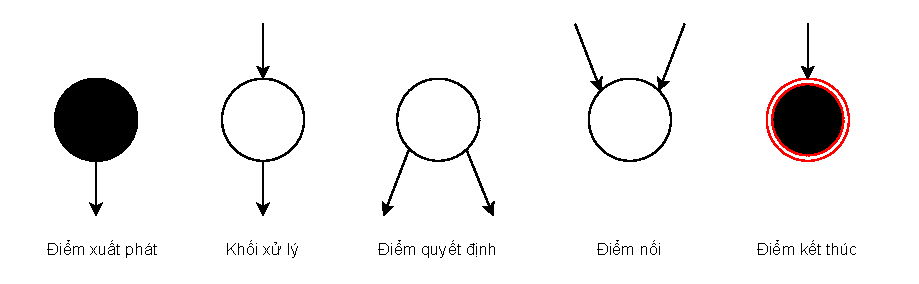
\includegraphics[width=1\columnwidth]{figures/c2/c2_cfg_point.drawio.pdf}
	\centering
	\caption{Các thành phần cơ bản trong đồ thị dòng điều khiển.}
	\label{img:background_cfg_point}
\end{figure}

\begin{figure}[H]
	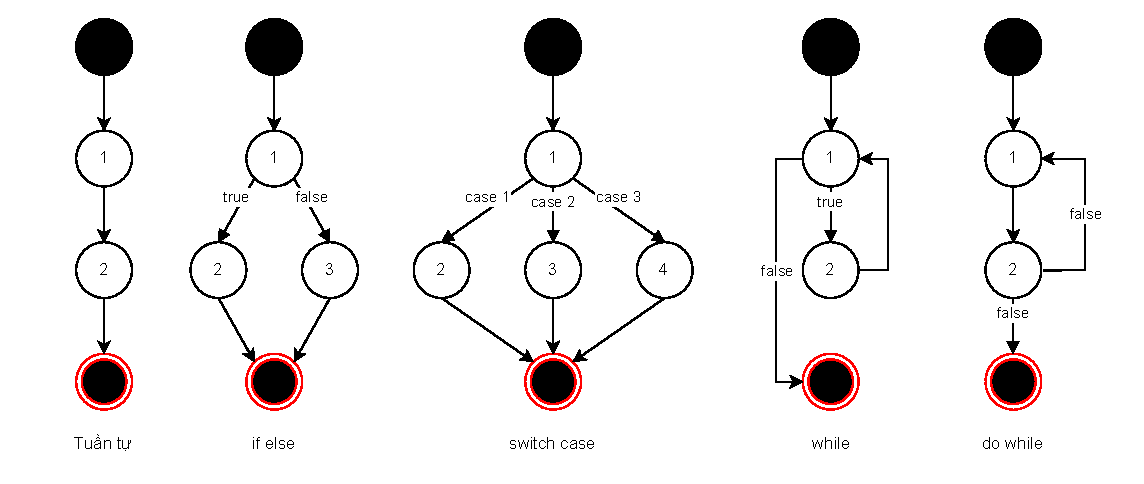
\includegraphics[width=1\columnwidth]{figures/c2/c2_cfg_line.drawio.pdf}
	\centering
	\caption{Các cấu trúc điều khiển phổ biến trong các ngôn ngữ lập trình.}
	\label{img:background_cfg_line}
\end{figure}

\begin{itemize}
  \item \textbf{Điểm xuất phát:} Đánh dấu thời điểm xuất phát của chương trình, được thể hiện bằng
  hình tròn đặc
  \item \textbf{Khối xử lý:} Đại diện cho các câu lệnh gán, khai báo và khởi tạo, được thể hiện bằng
  hình tròn rỗng;
  \item \textbf{Điểm quyết định:} Đại diện cho câu lệnh điều khiển trong khối lệnh điều khiển rẽ
  nhánh, được thể hiện bằng hình tròn rỗng và có nhiều cạnh đi ra từ điểm;
  \item \textbf{Điểm nối:} Đại diện cho câu lệnh được thực hiện ngay sau các lệnh rẽ nhánh, có
  nhiều hơn một điểm trỏ đến, được thể hiện bằng hình tròn rỗng;
  \item \textbf{Điểm kết thúc:} Đánh dấu thời điểm kết thúc của hàm, được thể hiện bằng hình tròn
  đặc có viền.
\end{itemize}

Hình 2.2 mô tả các cấu trúc điều khiển chính có trong mã nguồn C/C++ được mô phỏng dưới dạng các điểm của CFG, bao gồm có cấu trúc điều khiển tuần tự, rẽ nhánh if-else, switch-case, vòng lặp while c do ... và vòng lặp do ... while c.

\section{Đồ thị phụ thuộc chương trình}

Đồ thị phụ thuộc chương trình (Program Dependence Graph) biểu diễn chương
trình dưới dạng một đồ thị mà trong đó các nút là các câu lệnh và biểu thức (expression)
hoặc các toán tử và toán hạng. Các cạnh của đồ thị biểu diễn sự phụ thuộc dữ liệu (data
dependence) và điều kiện điều khiển (control condition) mà việc thực thi nút đó phụ
thuộc vào hay có thể hiểu đơn giản hơn là phụ thuộc điều khiển (control dependence)
[2].

\begin{figure}[H]
	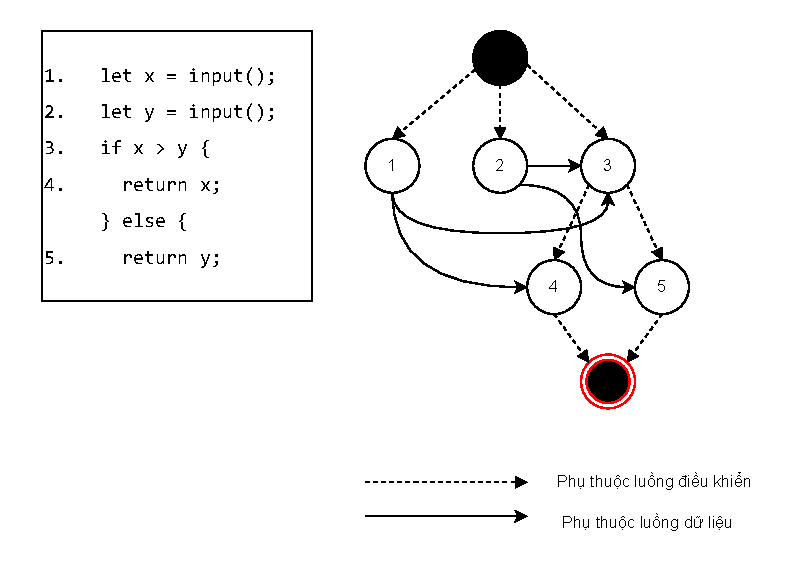
\includegraphics[width=1\columnwidth]{figures/c2/c2_pdg.drawio.pdf}
	\centering
	\caption{Ví dụ về đồ thị phụ thuộc chương trình}
	\label{img:background_pdg}
\end{figure}

Hình 2.4 biểu diễn ví dụ về một đồ thị phụ thuộc chương trình với nút ENTRY là
điểm bắt đầu của chương trình, các cạnh nét đứt biểu diễn phụ thuộc điều khiển và các
cạnh nét liền biểu diễn phụ thuộc dữ liệu.

\section{Đồ thị thuộc tính mã nguồn}

\textbf{NOTE:} Tự chạy 1 đoạn code sinh ra CPG rồi paste ảnh và đoạn code vào đây (thay cho ảnh và đoạn code bên dưới)

\begin{figure}[H]
	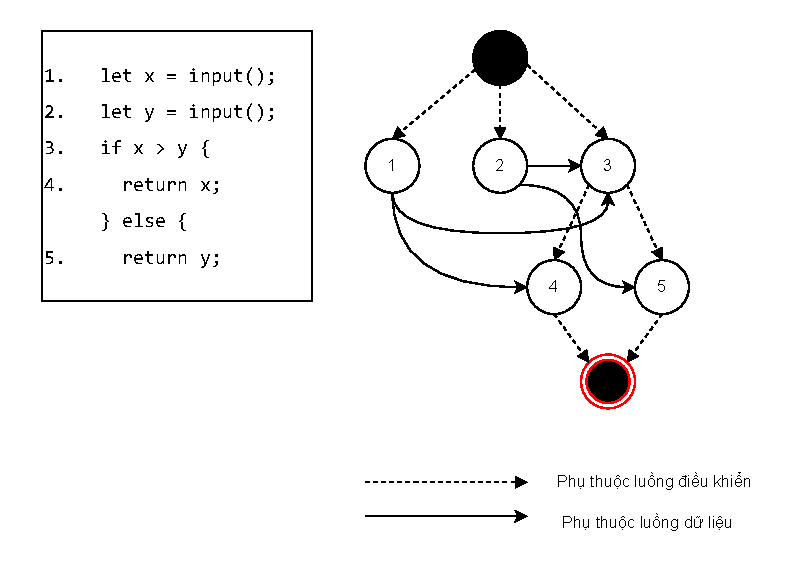
\includegraphics[width=1\columnwidth]{figures/c2/c2_pdg.drawio.pdf}
	\centering
	\caption{Đồ thị thuộc tính mã nguồn biểu diễn đoạn mã nguồn \ref{code:background_cpg}}
	\label{img:background_cpg}
\end{figure}

\begin{listing}[H]
\begin{minted}[mathescape, breaklines, frame=lines, framesep=2mm, baselinestretch=1.2, fontsize=\footnotesize, linenos]{rust}
fn main() {
  let x = input();
  let y = input();
  if x > y {
    return x;
  } else {
    return y;
  }
}
\end{minted}
\caption{Mã nguồn đầy đủ cho đồ thị thuộc tính mã nguồn \ref{img:background_cpg}}
\label{code:background_cpg}
\end{listing}

Đồ thị thuộc tính mã nguồn (Code Property Graph) là dạng đồ thị biểu diễn mã
nguồn của chương trình. Nó được hợp thành cây cú pháp trừu tượng, đồ thị dòng điều khiển và đồ thị phụ thuộc chương trình. Đồ thị chứa các thông tin về cấu trúc cú pháp,
luồng điều khiển và phụ thuộc dữ liệu trong chương trình. CPG được sử dụng để tìm
kiếm lỗ hổng trong mã nguồn, phát hiện sao chép mã nguồn, đo lường khả năng kiểm
thử mã nguồn và sinh mã khai thác. [7, 8, 11]

Các nút đại diện cho các thành phần như hàm, biến, lớp, gói và các cạnh đại diện
cho mối quan hệ giữa chúng như lời gọi hàm, sự gán giá trị, quan hệ cha con hay tham
chiếu.